\documentclass{article} % For LaTeX2e
\usepackage{nips12submit_e,times}
\usepackage{graphicx}
%\documentstyle[nips12submit_09,times,art10]{article} % For LaTeX 2.09


\title{Semi-Supervised Document Classification with Multinomial Naive Bayes}

%\linespread{1.0}

\author{
Christopher Clark \\
Department of Computer Science\\
University of Washington\\
Seattle, WA, 98195\\
\texttt{chrisc36@uw.edu}\\
\and
Coauthor Kevin Clark\\
Department of Computer Science\\
University of Washington\\
Seattle, WA, 98195\\
\texttt{kevinc22@uw.edu}\\
}

\newcommand{\fix}{\marginpar{FIX}}
\newcommand{\new}{\marginpar{NEW}}

\nipsfinalcopy % Uncomment for camera-ready version

\begin{document}


\maketitle

\begin{abstract}
We demonstrate how a text classifier can leverage a pool of unlabeled documents
to enhance classification performance.
Our technique uses Expectation-Maximization (EM) alongside a Multinomial Naive Bayes (MNB)
classifier. The classifier is trained on the labeled data and used to generated probabilistic labels for the unlabeled
data. The classifier is then trained using all the documents and regenerates label estimates for the unlabeled data.
This is repeated until convergence. We also investigate a similar semi-supervised extension to a MNB called Semi-supervised Frequency Estimation. Our results show that when labeled data is scarce
semi-supervision can increase classifier accuracy by up to 40\%.
\end{abstract}

\section{Introduction}
We focus on text classification, but the techniques discussed here could
generalize to other domains. Textual data is often abundant in places like digital records, electronic archives,
and company databases but labeling that data often must be done by hand. This can make training many
conventional algorithms overly expensive as labeling sufficient data for
these classifiers to achieve high accuracy is too costly. In this paper we
follow the approaches used by Nigam at al. [1] and Su et al. [2] to show how unlabeled data could be used to improve classifier
parameter estimation when there is little labelled data, reducing the need to label large numbers of examples.

\section{Multinomial Naive Bayes}
One common generative model for text classification is a Multinomial Naive Bayes classifier.
Consider classifying a list of documents as belonging to a set of discrete classes. We represent each document as a bag-of-words taken from a vocabulary $V$ consisting of
words $\langle{w_1,w_2...w_{|V|}}\rangle$. For a list of documents $D = \langle{d_1,d_2,...d_{|D|}\rangle}$, we represent a document $d_i$ as a
a vector of words counts $d_i = \langle{w_{i,1},w_{i,2}...w_{i,|V|}}\rangle$ where $w_{i,n}$ denotes the
number of times $w_n$ appears to $d_i$. We also have a list of potential classes for each document $Y = {\{y_1,y_2,...y_{|Y|}\}}$. To facilitate our EM
integration we generalize the standard algorithm by allowing the documents to have mixed membership. Thus
for a every document $d_i$ we assume we have a list $\langle{c_{i,1},c_{i,2},..c_{i,{|Y|}}\rangle}$ where
$c_{i,n}$ denotes the responsibility of membership class $y_n$ has on document $d_i$. When considering labeled data,
for any document $d_i$ labeled $y_j$ we set ${c_{i,k} = 1}$
if $k = j$ and ${c_{i,k} = 0}$ if $k \neq j$.


A MND is determined by a set of parameters we denote as $\Theta$.
Let $\Theta_{w_t|y_j} = P(w_t|y_j;\Theta)$, in other words $\Theta_{w_t|c_j}$
represents the probability $w_t$ appears in a document of class $y_j$. A MNB model also includes
a set of priors for each class written as $\Theta_{y_j}$.
Training a MNB consists of estimating the parameters to $\Theta$ given a list of documents and list of labels.

We estimate $\Theta$ by setting:
\[\Theta_{y_j}= {{ \sum_{i=1}^{|D|}c_{i,j}}\over{|D|}}, \ \ \ \ \ \ \Theta_{w_j|y_j} = {k + \sum_{i=1}^{|D|}c_{i,j}w_{i,j}\over{|V| * k + \sum_{n=1}^{|D|}\sum_{v=1}^{|v|}c_{i,j}w_{i,v}}}\]
where $k$ is a smoothing parameter. Now for an unlabeled document $d_k$ using a given $\Theta$ we can calculate:
\[P(y_j | d_k, \Theta) = \Theta_{y_j}\prod_{i=1}^{|V|}(\Theta_{w_i|y_j})^{w_{k,i}}\]
For classification purposes we can predict a class $\hat{c_k}$ for $d_k$ by setting:
\[\hat{c_k} = \arg\max_{y_j}P(y_j | d_k, \Theta) = \arg\max_{y_j}(\log(\Theta_{y_j}) + \sum_{i=1}^{|V|}\log(\Theta_{w_i|y_j})*w_{k,i})\]

\section{Using EM to Incorporate Unlabeled Data}
The first step of our algorithm is to build a standard MNB using the labeled data only to get an initial estimate of $\Theta$, $\hat{\Theta}$. Next we use Expectation Maximization to leverage the unlabeled data to improve our model's parameters. We do this following standard EM procedure
except we do not alter the label of the labeled data in the E-step. Particularly:

\begin{itemize}
\item E-step. We calculate a mixed membership label prediction for the unlabeled data. For a document $d_k$:
\[\forall j \in \{1,2,3...|Y|\} c_{k,j} = {P(y_j | d_k, \hat{\Theta}) \over {\sum_{n=1}^{|Y|} P(y_n | d_k, \hat{\Theta})}}\]

\item M-step. We reestimate $\hat{\Theta}$ using both the labelled and unlabeled examples.
\end{itemize}
We repeat the E-step and M-step until $\hat{\Theta}$ converges.

Since there are usually many more labeled than unlabeled examples, the unlabeled documents can dominate the EM and skew the parameter estimates. To fix this, we introduce a new parameter $\lambda$ determining the weight unlabeled documents. We set $\lambda=0.5$, which we found to provide good results in the experimental evaluation. A further step would be to take the approach of Nigam et al. [1] and determine the optimal value by performance on the validation set.

\section{Semi-supervised Frequency Estimation}
Semi-supervised Frequency Estimate (SFE) is a different extension to the MNB algorithm proposed by Su et al [2]. It runs like the EM algorithm described above except instead of using class membership probabilities for each document, it uses the class membership probabilities for each word obtained from the supervised learning. That is, $\Theta_{w_t|y_j}$ is set to
\[\Theta_{w_t|y_j} = {k + \sum_{i=1}^{|D|}P(c|w_i)_lw_{i,j}\over{|V| * k + \sum_{n=1}^{|D|}\sum_{v=1}^{|v|}P(c|w_i)_lw_{i,v}}}\].

Although this method performed worse than EM in our evaluation, there are other advantages to using this approach. Semi-supervised learning methods require large amounts of unlabeled data and thus need to scale well with the number of unlabeled documents. EM+MNB is a factor of $|C|$ slower than SF because EM requires a probability estimate for each unlabeled document belonging to each class while SF does not. Su et al. also found it outperformed EM on some data sets.

\section{Experimental Results}
We evaluated our classifier on the 20 Newsgroups data set, which consists of about 20,000 newsgroup documents divided almost evenly into 20 different UseNet discussion newsgroups. %The classification task is to determine which newsgroup a given article is posted in. 
We partitioned the data into four disjoint subsets: labeled training data (20\%), unlabeled training data (40\%), validation data (20\%), and test data (20\%). We varied the amount of labeled examples available to the classifier and recorded the classification accuracies of the MNB, SFE, and EM classifiers. In each case, the classifiers had access to all (roughly 7500) unlabeled examples. For smaller numbers of labeled training examples, we ran over multiple sets and averaged the results.

To select the smoothing parameter and the vocabulary, a grid search was performed on a validation set.  We found we got the best results when we converted all words to lowercase, removed stop words, removed words that
occurred only once, and removed words that occurred in over 50\% of the documents. We found $k = 0.40$
was the optimum smoothing parameter. 
\begin{figure}[h]
\begin{center}
%\framebox[4.0in]{$\;$}
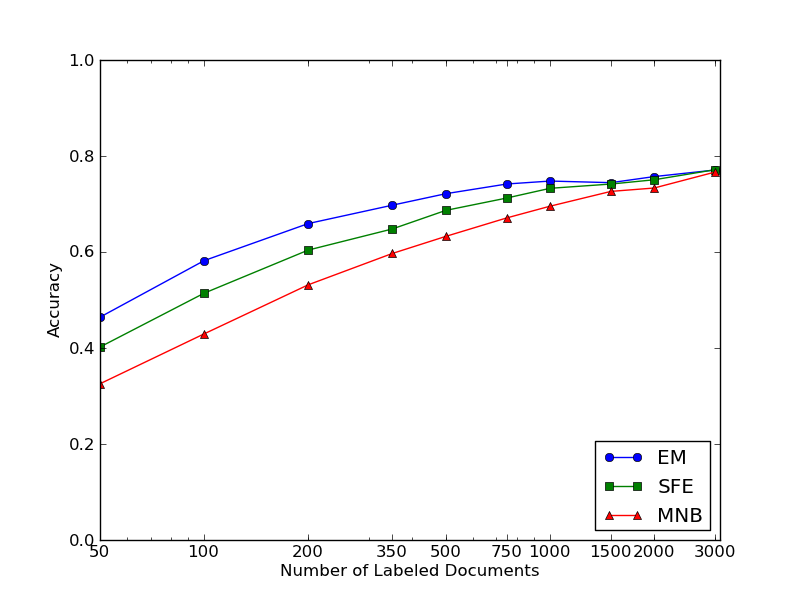
\includegraphics[width=3.06in]{results.png}
%\fbox{\rule[-.5cm]{0cm}{4cm} \rule[-.5cm]{4cm}{0cm}}
\end{center}
\caption{Classification accuracy on the 20 Newsgroups dataset}
\end{figure}

Using unlabeled data significantly boosted model performance, especially when the amount of training data. As the numbered of labeled examples increases, the gain from the additional data decreased, as the MNB could learn close to optimal parameters directly from the labeled data. 

\section{Future Work}
Our further work will focus on (1) building a more sophisticated model and (2) improving scalability. For (1) we will build a model with multiple mixture components per class, which will allow for better classification accuracy in cases where one class contains documents ranging over several topics. We also will compare the current model with co-training [3], another popular technique for semi-supervised learning. 

For (2), we will apply dimensionality reduction techniques, such as locality sensitive hashing and kernel hashing to produce more compact representations and smaller models. We also plan to parallelize the EM algorithm using MapReduce, allowing the algorithm to be run a distributed way. We will test performance over the DMOZ dataset, which is much larger than 20 Newsgroups. 

 \subsubsection*{References}
\small{
[1] Nigam, K., McCallum, A. K., Thrun, S., \& Mitchell, T. (2000) Text classification from labeled and unlabeled documents using EM. {\it Machine learning}, 39(2), 103-134.

[2] Su, J., Sayyad-Shirabad, J., \& Matwin, S. (2011) Large Scale Text Classification using Semi-supervised Multinomial Na�ve Bayes. ICML.

[3] Blum, A., \& Mitchell, T. (1998, July) Combining labeled and unlabeled data with co-training. In {\it Proceedings of the eleventh annual conference on Computational learning theory} (pp. 92-100). ACM. 

}



\end{document}



